\documentclass[12pt,aspectratio=43]{beamer}

%%%%%%%%%%%%%%%%%%%%%%%%%%%%%%%%%%%%%%%%%%%%%%%%%%
%   Paquetes de configuración basica del texto   %
%%%%%%%%%%%%%%%%%%%%%%%%%%%%%%%%%%%%%%%%%%%%%%%%%%
\usepackage[spanish,es-nodecimaldot]{babel}
\usepackage{biblatex}
\usepackage[T1]{fontenc}
\usepackage{listings}
\usepackage{multirow}
\usepackage{hyperref}
\usepackage{hyperxmp}
\usepackage{ifthen}
\usepackage{csquotes}

%%%%%%%%%%%%%%%%%%%%%%%%%%%%%%%%%%%%%%%%%%%%%%%%%%
%                   [listings]                   %
%   Configuración de vizualizacion del código    %
%%%%%%%%%%%%%%%%%%%%%%%%%%%%%%%%%%%%%%%%%%%%%%%%%%
\lstset{
	backgroundcolor=\color{lightgray!10},
	basicstyle=\ttfamily,
	extendedchars=true,
	showspaces=false,
	showstringspaces=false,
	captionpos=b,
	keywordstyle=\bfseries\color{cyan},
	commentstyle=\color{gray},
	stringstyle=\color{orange},
	escapeinside={!>}{<!},
	language=[LaTeX]TeX }

%%%%%%%%%%%%%%%%%%%%%%%%%%%%%%%%%%%%%%%%%%%%%%%%%%
%     Paquetes de configuración graficos del     %
%                   documento                    %
%%%%%%%%%%%%%%%%%%%%%%%%%%%%%%%%%%%%%%%%%%%%%%%%%%
\usepackage{graphicx}
\usepackage{tikz}
\usetikzlibrary{babel}
\usepackage{xcolor}
\usepackage{pdfpages}
\usepackage{animate}

\usepackage{ifxetex}
\ifxetex
	\usepackage[no-math]{fontspec}
	\setmainfont{AncizarSans}[
		Path = ../Fuentes/,
		Extension = .otf,
		BoldFont = *-B,
		ItalicFont = *-I,
		BoldItalicFont = *-BI ]
	\setmonofont{UbuntuMono}[
		Path = ../Fuentes/,
		Extension = .ttf,
		BoldFont = *-B,
		ItalicFont = *-I,
		BoldItalicFont = *-BI ]
	\newcommand{\lmr}{\fontfamily{lmr}\selectfont}
	\newcommand{\lmss}{\fontfamily{lmss}\selectfont}
	\newcommand{\lmtt}{\fontfamily{lmtt}\selectfont}
\fi

%%%%%%%%%%%%%%%%%%%%%%%%%%%%%%%%%%%%%%%%%%%%%%%%%%
%           Configuraciones de Beamer            %
%%%%%%%%%%%%%%%%%%%%%%%%%%%%%%%%%%%%%%%%%%%%%%%%%%
\definecolor{Igreen}{RGB}{148,180,59}
\definecolor{Ired}{RGB}{166,24,49}

\setbeamertemplate{navigation symbols}{}

\setbeamertemplate{itemize items}{\color{Igreen}\raisebox{.45ex}{\rule{.6ex}{.6ex}}}
\setbeamertemplate{enumerate item}{\color{Igreen}\bfseries\arabic{enumi}.}
\setbeamertemplate{enumerate subitem}{\color{Igreen}\bfseries\arabic{enumi}.\arabic{enumii}.}

\usefonttheme{professionalfonts}
\usefonttheme{serif}

\setbeamercolor{frametitle}{fg=Ired,bg=Igreen!50}
\setbeamercolor{alerted text}{fg=Ired}

\setbeamertemplate{bibliography item}{
	\ifboolexpr{ test {\ifentrytype{book}} or test {\ifentrytype{mvbook}}
		or test {\ifentrytype{collection}} or test {\ifentrytype{mvcollection}}
		or test {\ifentrytype{reference}} or test {\ifentrytype{mvreference}} }
	{\setbeamertemplate{bibliography item}[book]}
	{\ifentrytype{online}
		{\setbeamertemplate{bibliography item}[online]}
		{\setbeamertemplate{bibliography item}[article]}}
	\usebeamertemplate{bibliography item}}

\defbibenvironment{bibliography}
	{\list{}
		{\settowidth{\labelwidth}{\usebeamertemplate{bibliography item}}%
			\setlength{\leftmargin}{\labelwidth}%
			\setlength{\labelsep}{\biblabelsep}%
			\addtolength{\leftmargin}{\labelsep}%
			\setlength{\itemsep}{\bibitemsep}%
			\setlength{\parsep}{\bibparsep}}}
	{\endlist}
	{\item}

\makeatletter
\newcommand{\ifratio}[2]{
	\ifthenelse
	{\lengthtest{\beamer@paperwidth=16cm} \AND \lengthtest{\beamer@paperheight=9cm}}
	{#1}
	{#2} }
\makeatother

\setbeamertemplate{title page}{
	\begin{tikzpicture}[overlay,remember picture]
	\path (current page.north west) ++(0.5cm,-0.5cm) node[below right] {
\includegraphics[height=1.25cm]{../Escudo_UN}};
	\path (current page.north east) ++(-0.5cm,-0.5cm) node[below left] {\parbox[c][1.25cm][c]{\widthof{\Large \insertsubtitle}}{\Large \insertsubtitle}};
	\end{tikzpicture}

	\vfill
	\begin{center}
		{\Huge\inserttitle}\\
		\bigskip
		\insertauthor
	\end{center}
	\vfill
}

%%%%%%%%%%%%%%%%%%%%%%%%%%%%%%%%%%%%%%%%%%%%%%%%%%
%         Información de la presentación         %
%%%%%%%%%%%%%%%%%%%%%%%%%%%%%%%%%%%%%%%%%%%%%%%%%%

\title{{\lmr\LaTeX} en móviles}
\subtitle{Curso Libre de {\lmr\LaTeX}}
\author{Joar Esteban Buitrago Carrillo}
\institute{Universidad Nacional de Colombia}
\date{}
\logo{
\includegraphics[height=0.75cm]{../Escudo_UN}}
\hypersetup{
	pdfcopyright={Esta obra está bajo una licencia de Creative Commons Reconocimiento-CompartirIgual 4.0 Internacional.},
	pdflicenseurl={https://creativecommons.org/licenses/by-sa/4.0/deed.es}
}
\addbibresource{biblio.bib}

\begin{document}
\begin{frame}[plain]
\titlepage
\end{frame}

{
\setbeamercolor{background canvas}{bg=}
\begin{frame}
\ifratio
	{\includepdf[pages=2]{../Licencia_Diapositiva.pdf}}
	{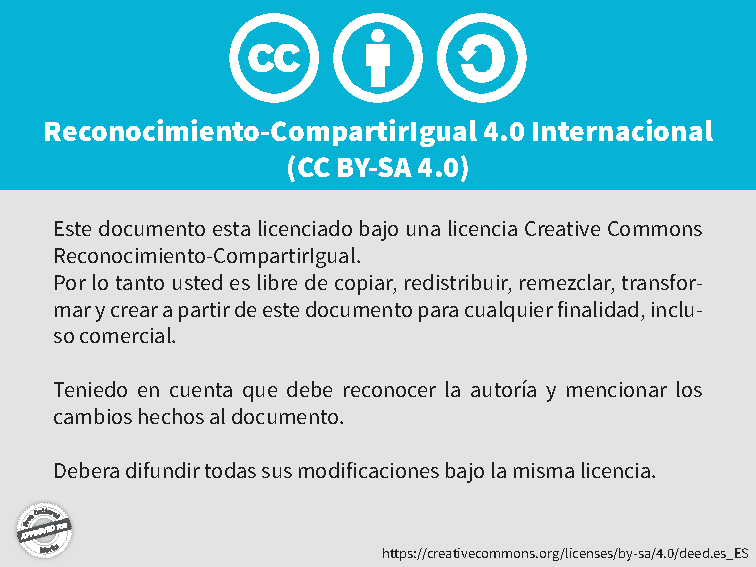
\includepdf[pages=1]{../Licencia_Diapositiva.pdf}}
\end{frame}
}

\section{Termux}
\begin{frame}{Termux}{}
\begin{center}
	
\includegraphics[height=3cm]{Termux_Logo}\hspace{1em}\parbox[b][3cm][c]{\widthof{\Huge Termux}}{\Huge Termux}
\end{center}

Página web: https://termux.com/
\end{frame}

\begin{frame}{Termux}{}
\alert{\bf Termux} es un potente emulador de terminal que funciona con Android aprovechando que este sistema operativo está basado en Linux.\pause\\[1em]

Este emulador tiene soporte a la mayoría de paquetes de Linux, incluyendo {\lmr\TeX} Live y muchos editores de texto como Emacs, Vim, micro, nano, etc. Nosotros utilizaremos Emacs ya que su manejo en este entorno se vuelve muy cómodo.
\end{frame}

\begin{frame}{Termux}{}
Para instalar Termux sólo debemos dirigirnos a la Play Store y descargarlo desde allí.\pause\\[1em]

Los administradores de paquetes de Termux son \texttt{pkg} y \texttt{apt}, lo cual hace que descargar e instalar paquetes sea muy rápido y eficiente.
\end{frame}

\begin{frame}[plain]
\begin{center}
	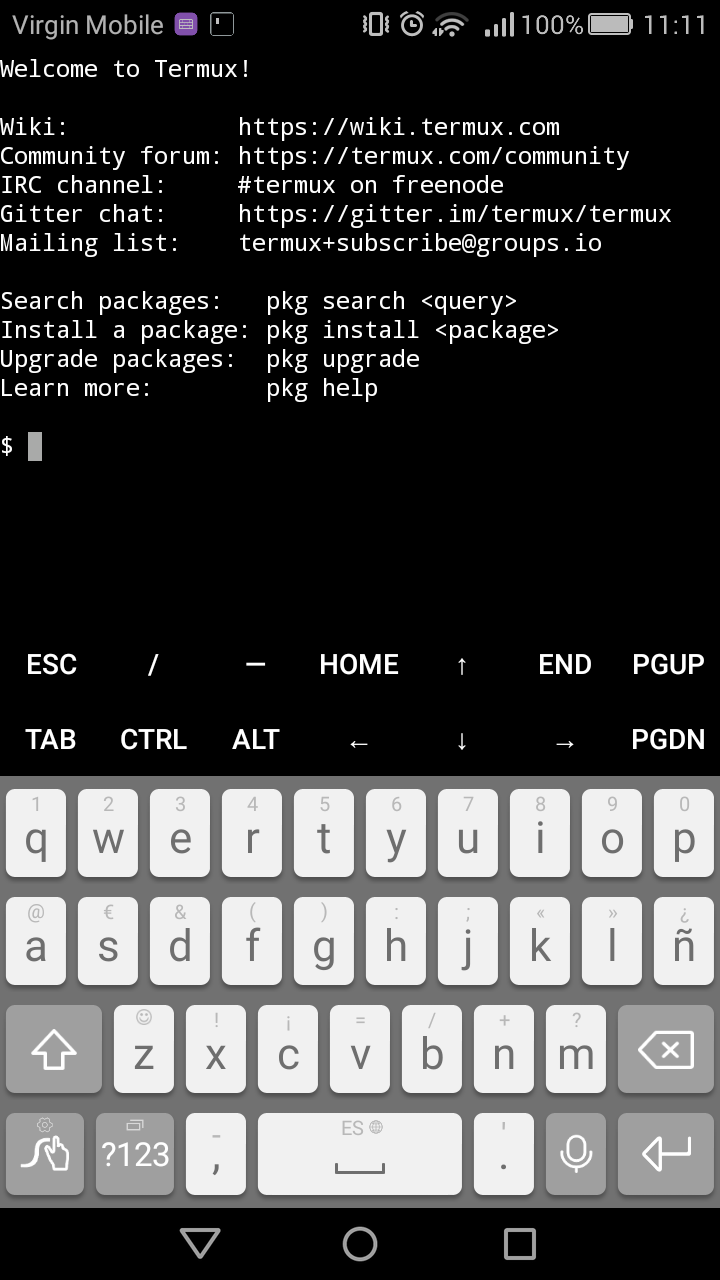
\includegraphics[height=0.9\textheight]{Screen_Blank}
\end{center}
\end{frame}

\section{Instalación de {\LaTeX}}
\begin{frame}{Instalación de {\lmr\LaTeX}}{}
Para instalar {\lmr\LaTeX} en Termux solo debemos escribir el comando\\[1em]

\texttt{apt install texlive}\pause\\[1em]

Tras lo cual se empezara la descarga e instalación de todos los paquetes requeridos para hacer que {\lmr\LaTeX} funcione.
\end{frame}

\section{Instalación de Emacs y AUCTeX}
\begin{frame}{Instalación de Emacs y AUC{\TeX}}{}
De igual manera, para instalar Emacs y AUC{\TeX} en Termux solo debemos escribir el comando\\[1em]

\texttt{apt install emacs}\pause\\[1em]

Tras lo cual se empezara la descarga e instalación de Emacs.
\end{frame}

\begin{frame}{Instalación de Emacs y AUC{\TeX}}{}
Una vez instalado Emacs podremos instalar AUC{\TeX} mediante MELPA. Entonces tocaremos Alt + M, y escribiremos \texttt{package-install} y damos al entrar.\pause\\[1em]

Después escribiremos AUC{\TeX} y Emacs empezara con la descarga e instalación de todos los paquetes de AUC{\TeX}.
\end{frame}

\begin{frame}[plain]
\begin{center}
	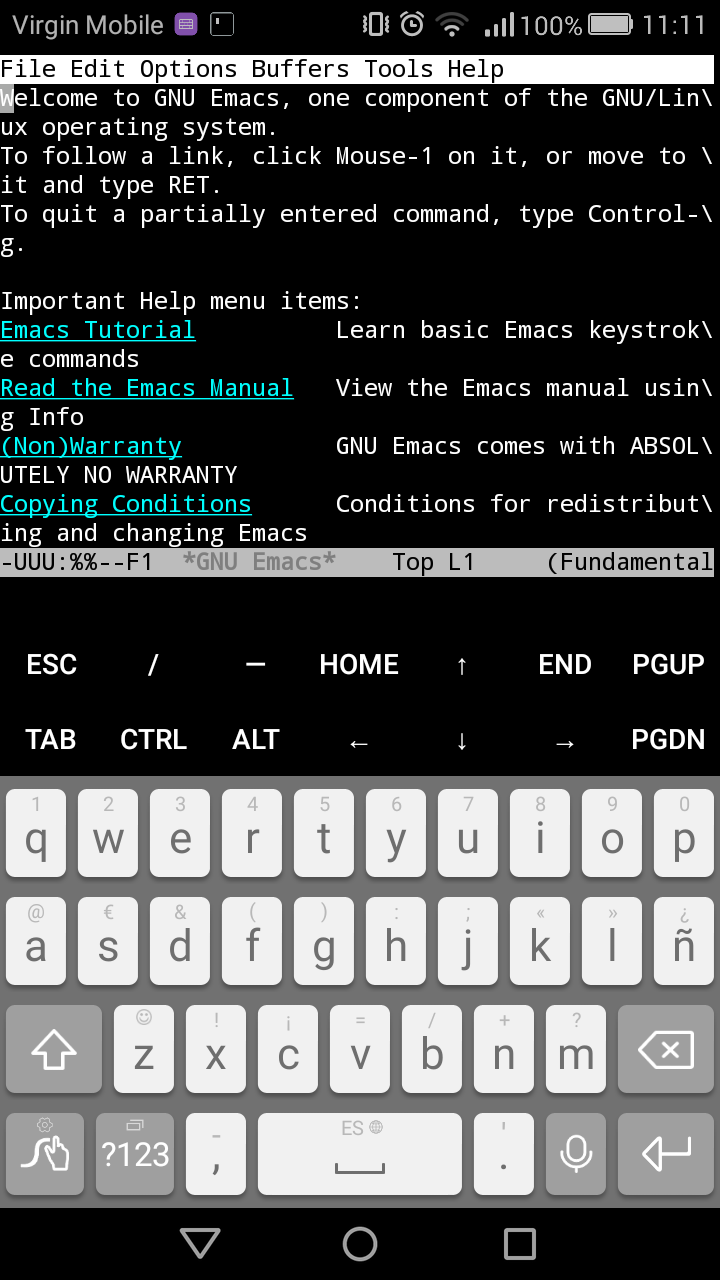
\includegraphics[height=0.9\textheight]{Screen_Emacs}
\end{center}
\end{frame}

\begin{frame}[plain]
\begin{center}
	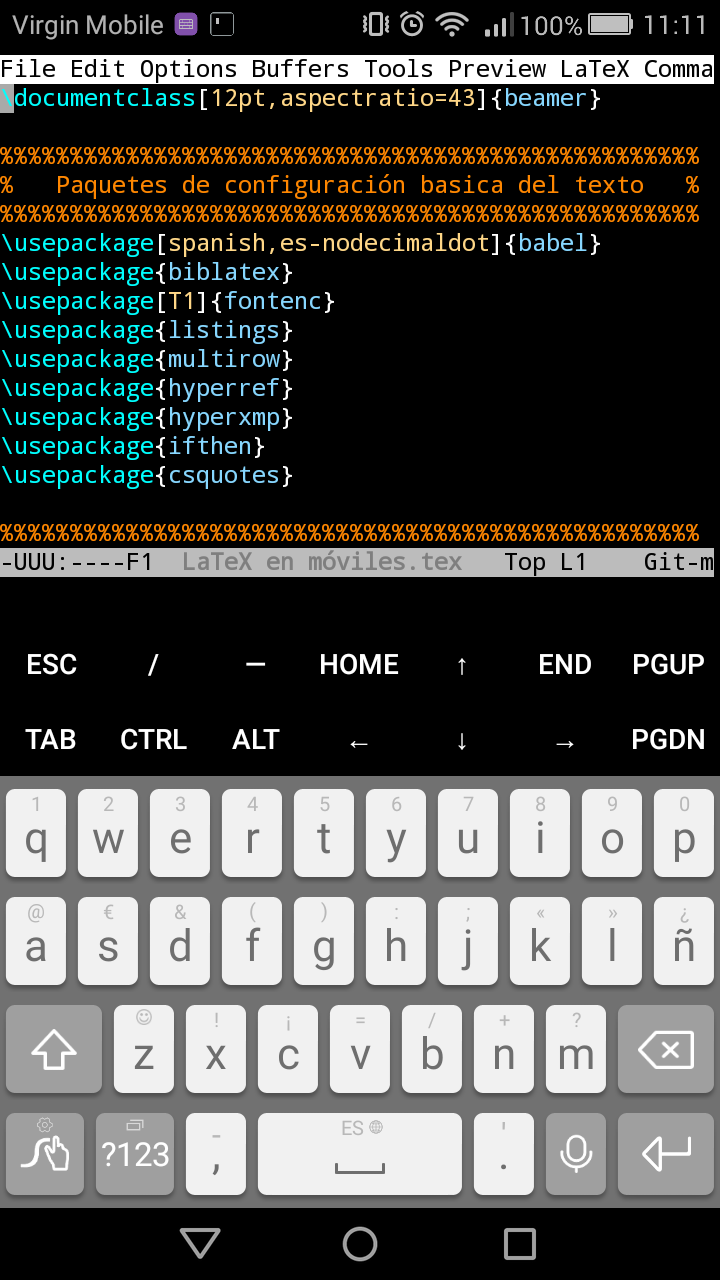
\includegraphics[height=0.9\textheight]{Screen_AUCTeX}
\end{center}
\end{frame}

\section{Instalación de paquetes}
\begin{frame}{Instalación de paquetes}{}
Para instalar los paquetes faltantes en {\lmr\TeX} Live, este incluye el comando \texttt{tlmgr} para la administración de estos.\pause\\[1em]

Para instalar un paquete sólo debemos de escribir\\[1em]

\texttt{tlmgr install <nombre del paquete>}\pause\\[1em]

Tras lo cuál {\lmr\TeX} Live descargara e instalará los paquetes indicados.
\end{frame}

\section{Actualización}
\begin{frame}{Actualización}{}
Para actualizar los paquetes, de manera similar debemos de escribir\\[1em]

\texttt{apt update}\\
\texttt{apt upgrade}\pause\\[1em]

Para actualizar los programas, como el editor y {\lmr\TeX} Live.\pause\\
Y debemos escribir\\[1em]

\texttt{tlmgr update --self --all}\\[1em]

Para actualizar los paquetes de {\lmr\LaTeX}.
\end{frame}

\section{Compilación}
\newcommand{\XeLaTeX}{\lmr X\hspace{-0.3ex}\raisebox{-0.5ex}{\reflectbox{E}}\hspace{-0.25ex}{\LaTeX}}
\begin{frame}{Compilación}{}
Cuando compilas un documento desde la \alert{\bf consola} solo debes de escribir el nombre de tu compilador favorito seguido del archivo \texttt{.tex} de {\lmr\LaTeX}.\pause\\[1em]

De esta forma entonces para compilar estas presentaciones utilizando {\XeLaTeX} será:\\[1em]

\texttt{xelatex "LaTeX en móviles.tex"}\pause\\[1em]

Aunque es bueno compilar el documento más de una vez, para que {\lmr\LaTeX} acomode bien todo en el texto.
\end{frame}

\begin{frame}[plain]
\begin{center}
	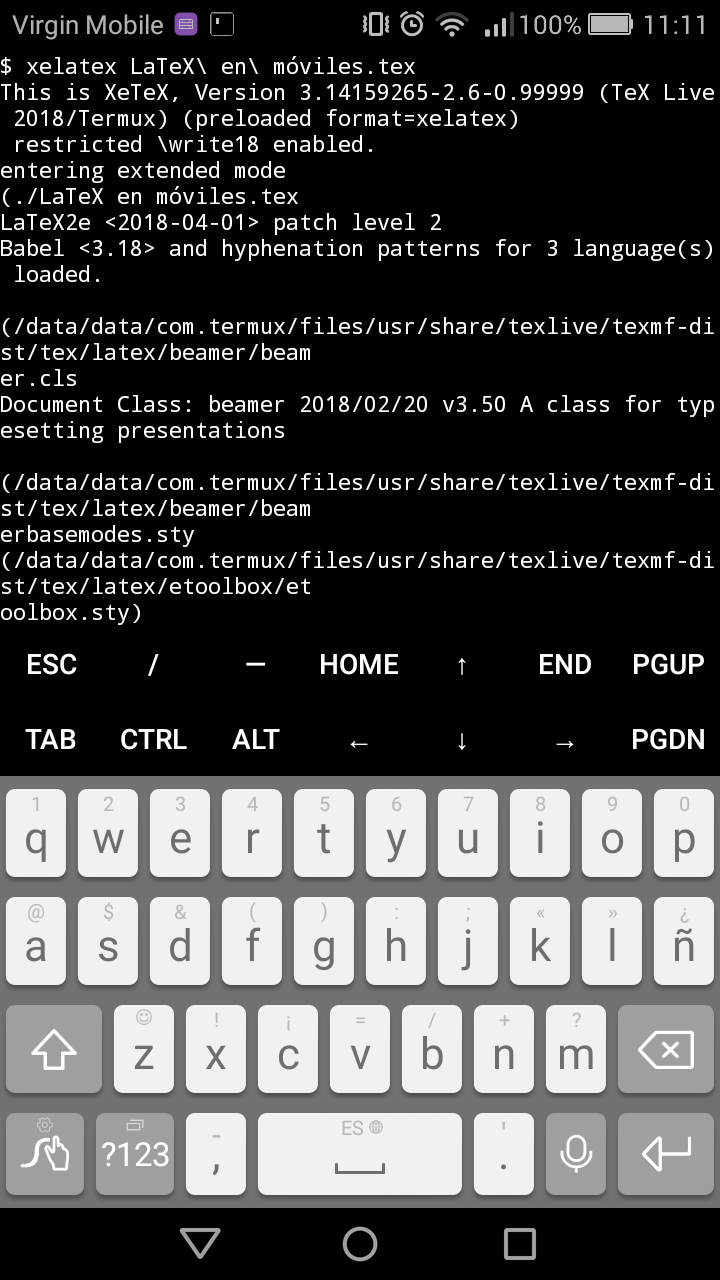
\includegraphics[height=0.9\textheight]{Screen_Compile_1}
\end{center}
\end{frame}

\begin{frame}[plain]
\begin{center}
	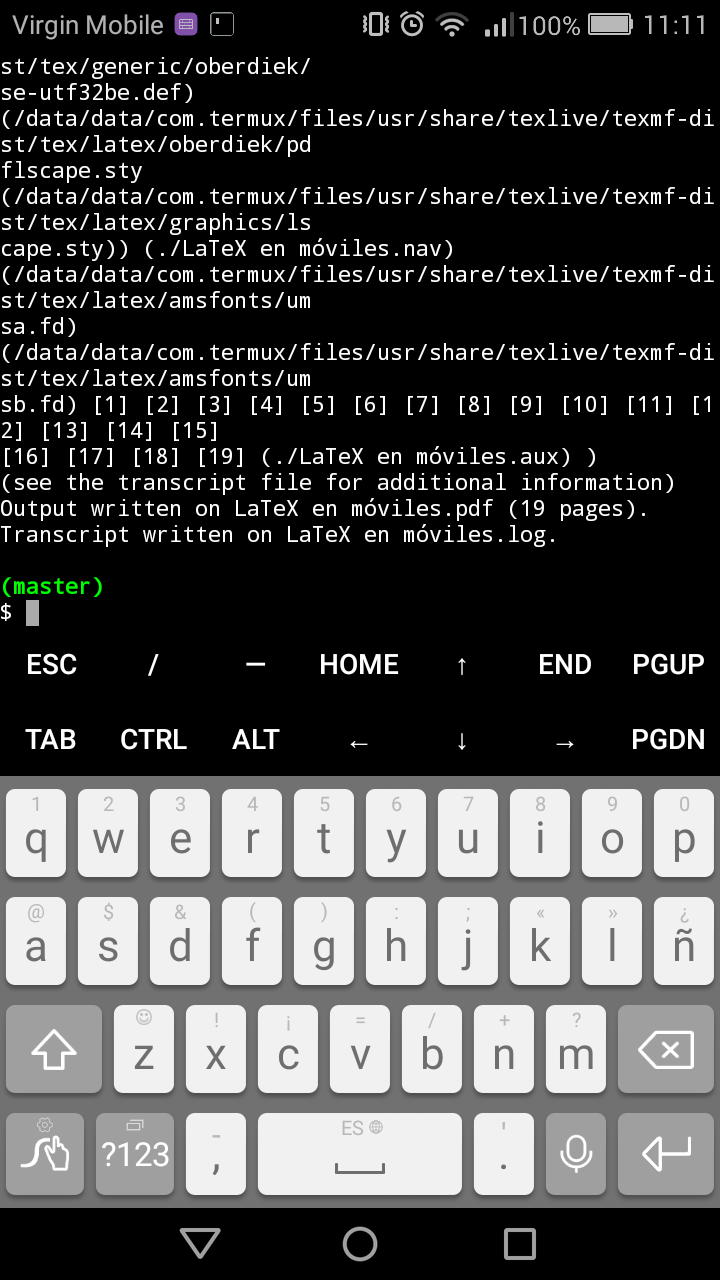
\includegraphics[height=0.9\textheight]{Screen_Compile_2}
\end{center}
\end{frame}

\begin{frame}{Compilación}{}
Para compilar con AUC{\TeX} debes oprimir dos veces \texttt{Ctrl} + \texttt{C} y escribir \texttt{LaTeX}, tras lo cual empezara la compilación en segundo plano.\pause\\[1em]

En caso de querer ver el trabajo de compilación puedes oprimir \texttt{Ctrl} + \texttt{C} y \texttt{Ctrl} + \texttt{L}.\pause\\[1em]

Una vez la compilación termine AUC{\TeX} te dira si es necesario compilar de nuevo, recordando que es mejor si el documento se compila más de una vez.
\end{frame}

\begin{frame}[plain]
\begin{center}
	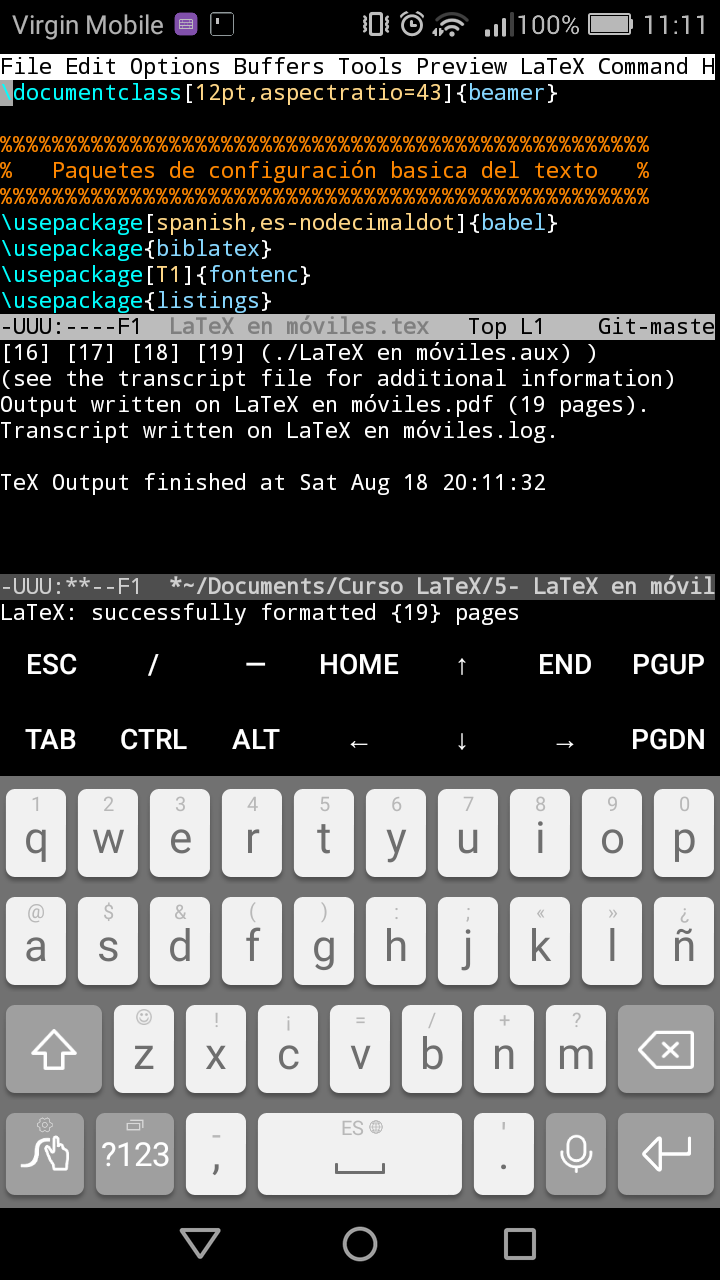
\includegraphics[height=0.9\textheight]{Screen_AUCTeX_Compile_1}
\end{center}
\end{frame}

\begin{frame}[plain]
\begin{center}
	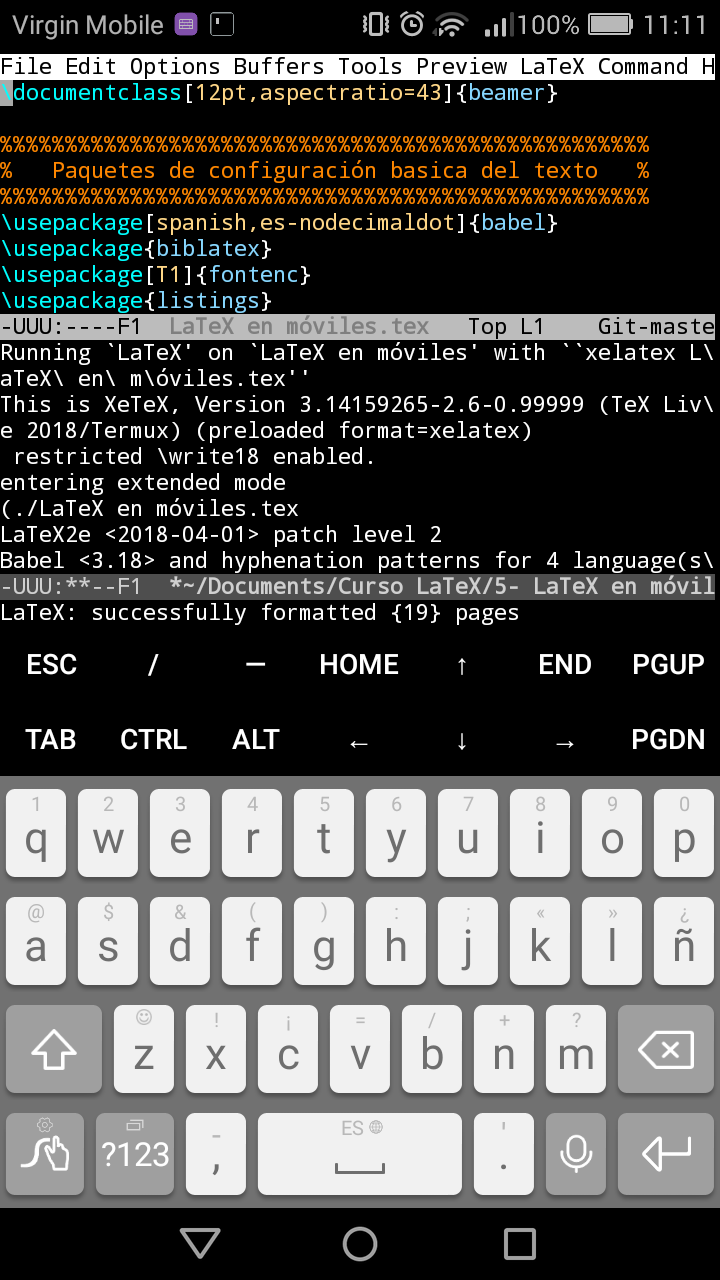
\includegraphics[height=0.9\textheight]{Screen_AUCTeX_Compile_2}
\end{center}
\end{frame}

\begin{frame}{Bibliografía}
\nocite{*}
\printbibliography
\end{frame}
\end{document}
